\documentclass{article}
\usepackage[a4paper, total={7in, 10in}]{geometry}
\usepackage{fontspec} 
\usepackage{xeCJK} 
\setCJKmainfont{標楷體}
\setmainfont{Times New Roman}
\XeTeXlinebreaklocale “zh” 
\XeTeXlinebreakskip = 0pt plus 1pt
\usepackage{graphicx}
\usepackage{float}
\usepackage{xcolor}
\usepackage[linesnumbered,ruled,vlined]{algorithm2e}
\usepackage{mathtools}
\usepackage{amsmath} 
\usepackage{subfigure}  




\newcommand\mycommfont[1]{\footnotesize\ttfamily\textcolor{blue}{#1}}
\SetCommentSty{mycommfont}

\SetKwInput{KwInput}{Input}                % Set the Input
\SetKwInput{KwOutput}{Output}              % set the Output

\title{Self-Driving Cars}
\author{309611087 洪得瑜}
\date{2022 10/20} 

\begin{document}
\maketitle
\section{Kalman Filter}
\begin{itemize}
	\item Introudction
	\item Briefly explain your code
	\item Include the ouput Image
	\item How you design the covariance matrices(Q, R)?
	\item How will the value of Q and R affect the output of Kalman filter?
\end{itemize}
\subsection{Implement}
\begin{document}
\subsubsection{Init\cite{2}}
\begin{enumerate}
	\item $x$ 為狀態矩陣包含[x y yaw] 初始值設定為[0 0 0]
	\item $A$ 為狀態轉換矩陣它將時間 t-1 的每個系統狀態參數的影響應用於時間 t 的系統狀態在這設定為I
	\item $u_t$為控制參數如油門或者位置控制等
	\item $B$ 為輸入控制矩陣將$u_t$的控制參數影響狀態向量
	\item $P$ 為協方差矩陣(Error matrx)對角線為是狀態向量中對應相關方差,非對角項為狀態向量之間的協方差,在這初始設定為I彼此獨立,下一時刻會更新新的協方矩陣
	\item $H$ 為狀態向量轉換到量測向量轉換矩陣在這設定$\begin{bmatrix}1 & 0 & 0\\0 & 1 & 0\end{bmatrix}$,因此對於yaw並不影響量測狀態
	\item $Q$ 矩陣為狀態協方矩陣和控制noisy有關,影響predict,在這控制項為3項因此為3X3矩陣
	\item $R$ 矩陣為量測noisy協方矩陣,量測結果為x 及 y因此為2X2矩陣
\end{enumerate}
\begin{figure}[H]
\begin{center}
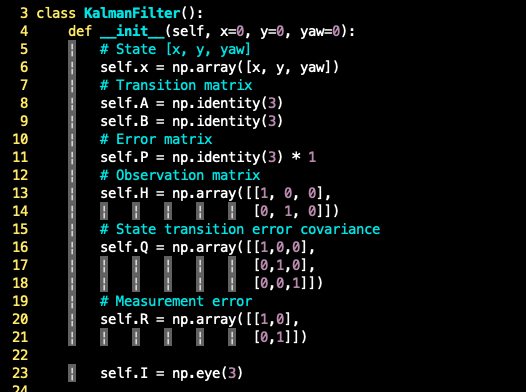
\includegraphics[scale=0.5]{code.png}
\caption{程式初始化}
\end{center}
\end{figure}
\subsubsection{Predict}
基於動態方程估測下一時刻狀態,為當前狀態加上控制向量與動態矩陣轉換下一狀態差生成下ㄧ刻狀態預測,並計算下一時刻$P$誤差矩陣,之後呼叫Update函數進行filter ,演算法如1所示。\\
\\
\\
演算法參數對照程式碼:\\
$F=A$\\
$B=B$\\
$u=u$\\
$P=P$\\
$Q=Q$ 需要tuning \\
\begin{algorithm}[H]
\DontPrintSemicolon
\KwInput{state $x$ , control $u$}
\KwOutput{new state$\hat{x}$ ,$ P$}
$\hat{x}=Fx+Bu$ \\
$P=FPF^T+Q$ \\
\label{alg:predict}
\caption{Predict\cite{1}}
\end{algorithm}
轉換成程式碼:\\
\begin{figure}[H]
\begin{center}
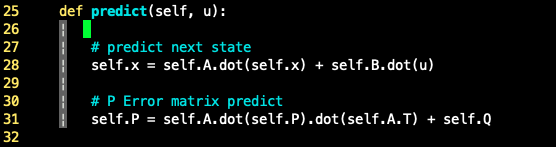
\includegraphics[scale=0.5]{code2.png}
\caption{Predict函數}
\end{center}
\end{figure}
\subsubsection{Update}

經由前一時刻預測後的狀態與當前的狀態透過Kalman gain($K$)調整weight重新計算出當前新的狀態,並更新至 $x$ 狀態及新的$P$協方矩陣,演算法如2所示。 \\
程式碼對照演算法:\\
\begin{enumerate}
	\item 參數$H=H$,$R$需要tuning
	\item 計算$K$分兩階段計算$S$為$(HPH^T+R)^{-1}$
	\item 計算出$K=PH^TS^{-1}$
	\item $\hat{y}$對照程式$y$為計算量測狀態與預測狀態margin,程式碼為$y=z-Hx$
	\item 重新計算狀態$x=x+Ky$,由前步驟可得$K,y$
	\item $P=(I-KH)P$ 和程式碼不同原因在於此方程式假設K值為最佳值,但實際應用上並非總能計算出最優解,所以應用上修改為$P=(I-KH)P(I-KRK)^T+KRK^T$,讓數值能更加穩定但缺點在於需要增加計算量,經測試在本次作業兩者並無顯著差異\cite{1}。
\end{enumerate}
\begin{algorithm}[H]
\DontPrintSemicolon 
\KwInput{$\hat{x}$ $P$ $z$}
\KwOutput{$\hat{x}$ $P$}
  $\hat{y}$ = $z - H\hat{x}$ \\
  $K=PH^T(HPH^T+R)^{-1}$ \\
  $\hat{x}=\hat{x}+K\hat{y}$ \\
  $P=(I-KH)P$ \\
  \Return $\hat{x}$ , P
  \caption{Update\cite{1}}
\end{algorithm}
\begin{figure}[H]
\begin{center}
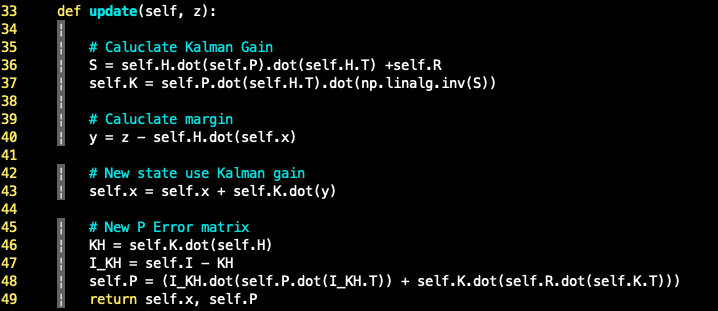
\includegraphics[scale=0.5]{code3.png}
\caption{Update函數}
\end{center}
\end{figure}
\subsection{Q R tuning}
$Q$及$R$矩陣各別為協方差矩陣可定義為如下:\\
$Q=
\begin{bmatrix}
	{\sigma_x}^2 & cov(x,y) & cov(x,z) \\
	cov(y,x) & {\sigma_y}^2 & cov(y,z)\\
	cov(z,x) & cov(z,y) & {\sigma_z}^2\\
\end{bmatrix}$
$R=\begin{bmatrix}
	{\sigma_x}^2 & \rho\sigma_x\sigma_y \\
	\rho\sigma_y\sigma_x & {\sigma_y}^2
\end{bmatrix}$\\
\\
Control term : mean = 0 , var = 0.1\\
\\
Measrement : mean = 0, var = 0.75\\
\\
\subsubsection{Analyze 1}
	將Q R 矩陣皆初始設定為單位矩陣與已知輸入variance,則Q = I*0.1 及 R = I*0.75 ,進行比較分析結果顯示以Q = I*0.1 及 R = I*0.75結果較佳,能有效抑制雜訊且由矩陣看出量測所造成的雜訊,結果如圖下所示。
\begin{figure}[H]
	\centering
	\subfigure[Q R 為單位矩陣]{
		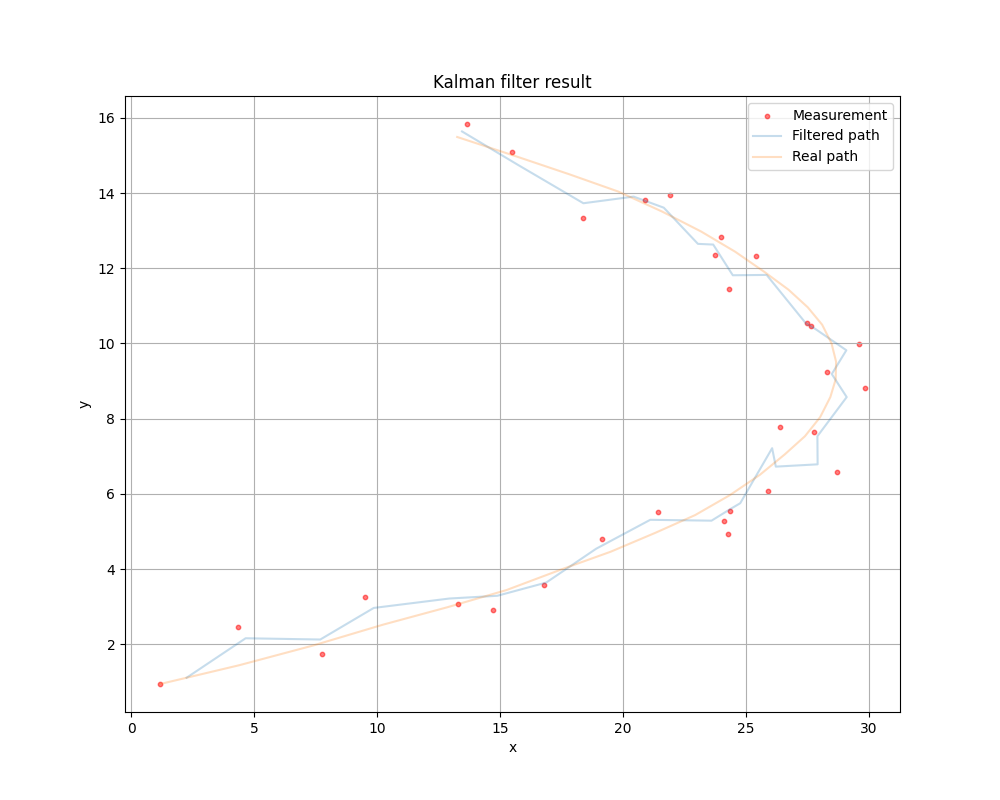
\includegraphics[width=0.4\textwidth]{./org/Figure_1.png}
	}
	\subfigure[Q R 以已知var做設計有效降低雜訊]{
		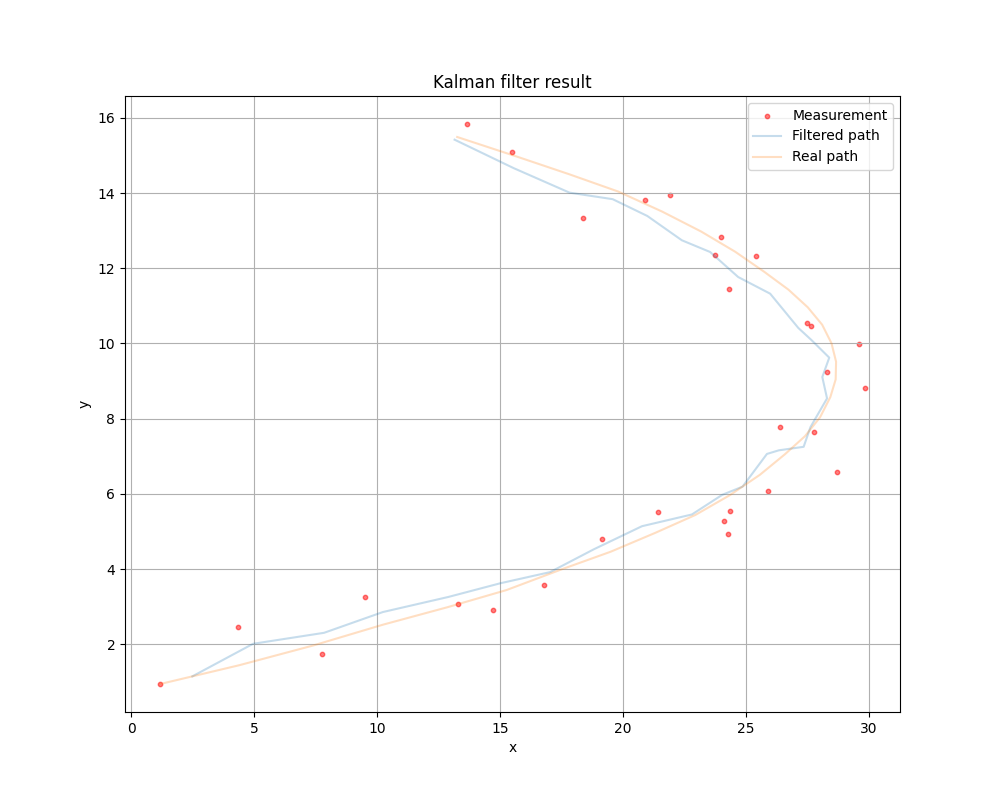
\includegraphics[width=0.4\textwidth]{./org/Figure_2.png}
	}
\end{figure}


\subsubsection{Analyze 2}
分析2以固定$Q=\begin{bmatrix} 0.1 & 0 & 0\\ 0 & 0.1 & 0\\ 0 & 0 & 0.1 \end{bmatrix}$,調整R$\begin{bmatrix} 0.75 & \rho*0.75\\ \rho*0.75 & 0.75 \end{bmatrix}$矩陣中的$\rho$分析量測變異數x 和 y 之間相關性,設定條件$-1 < \rho < 1 $之間依序調整驗證相關性,經驗證結果$\rho=0$最接近ground truth所以在量測雜訊中x y 為非相關,結果如圖下所示。
\begin{figure}[H]
\centering
	\subfigure[$\rho=0.99$]{
	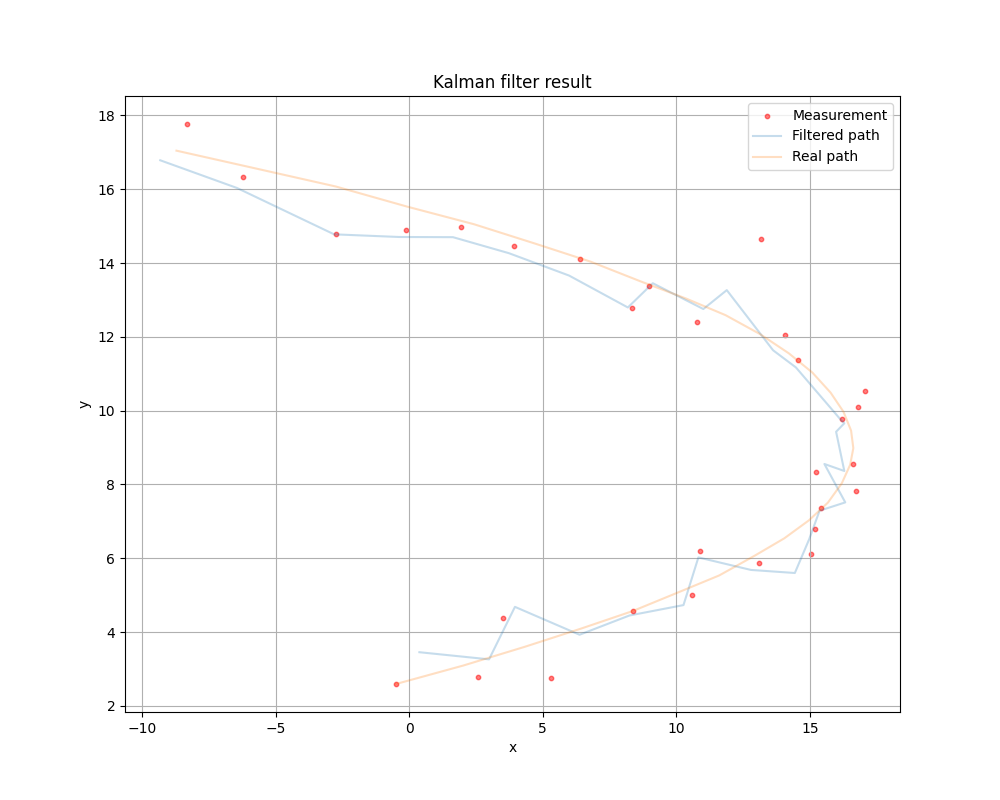
\includegraphics[width=0.4\textwidth]{./analyze1/Figure_1.png}
	}
	\subfigure[$\rho=0.5$]{
		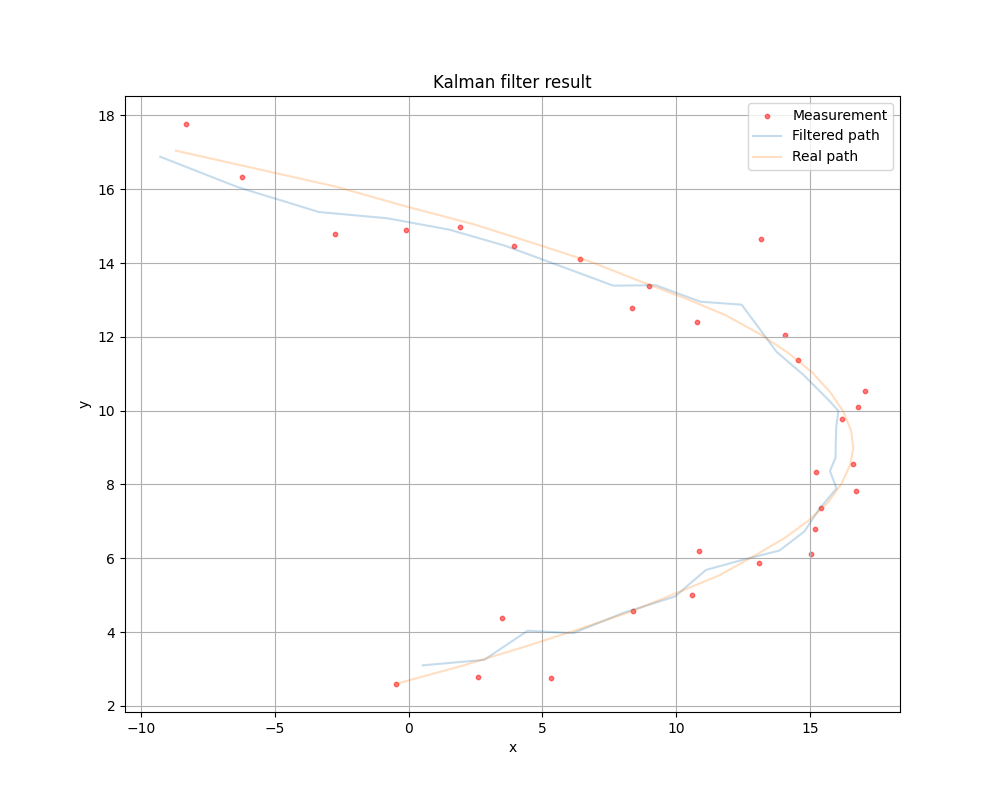
\includegraphics[width=0.4\textwidth]{./analyze1/Figure_2.png}
	}
\end{figure}
\begin{figure}[H]
	\centering
	\subfigure[$\rho=0$]{
		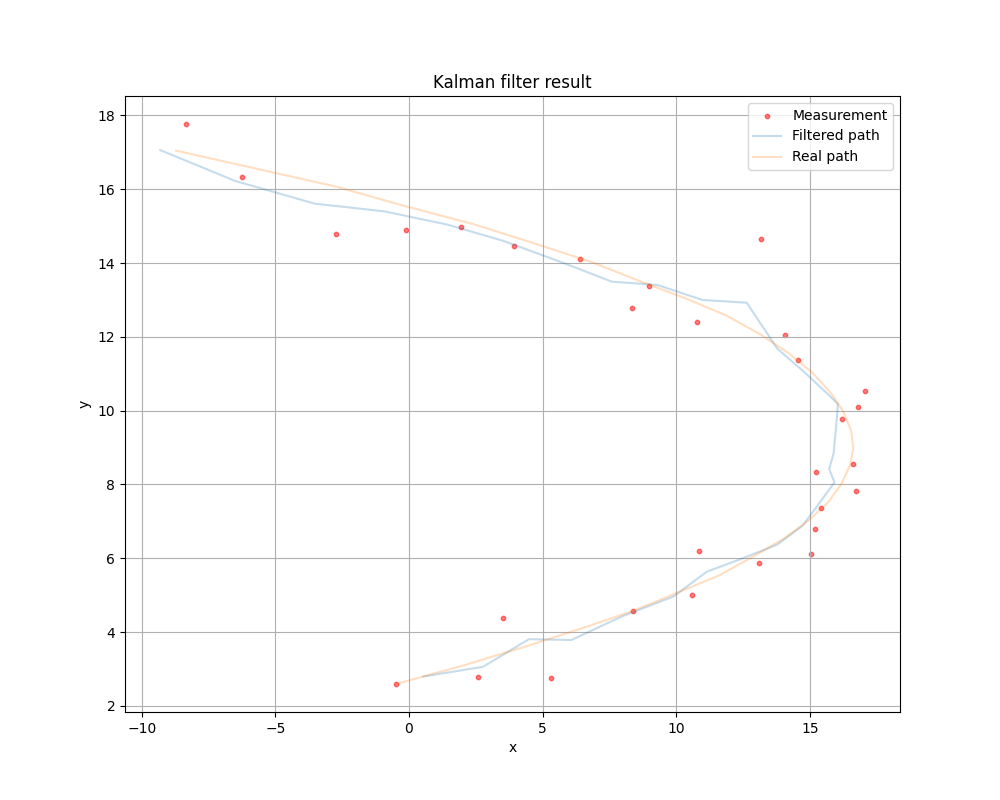
\includegraphics[width=0.4\textwidth]{./analyze1/Figure_3.png}
	}
	\subfigure[$\rho=-0.5$]{
		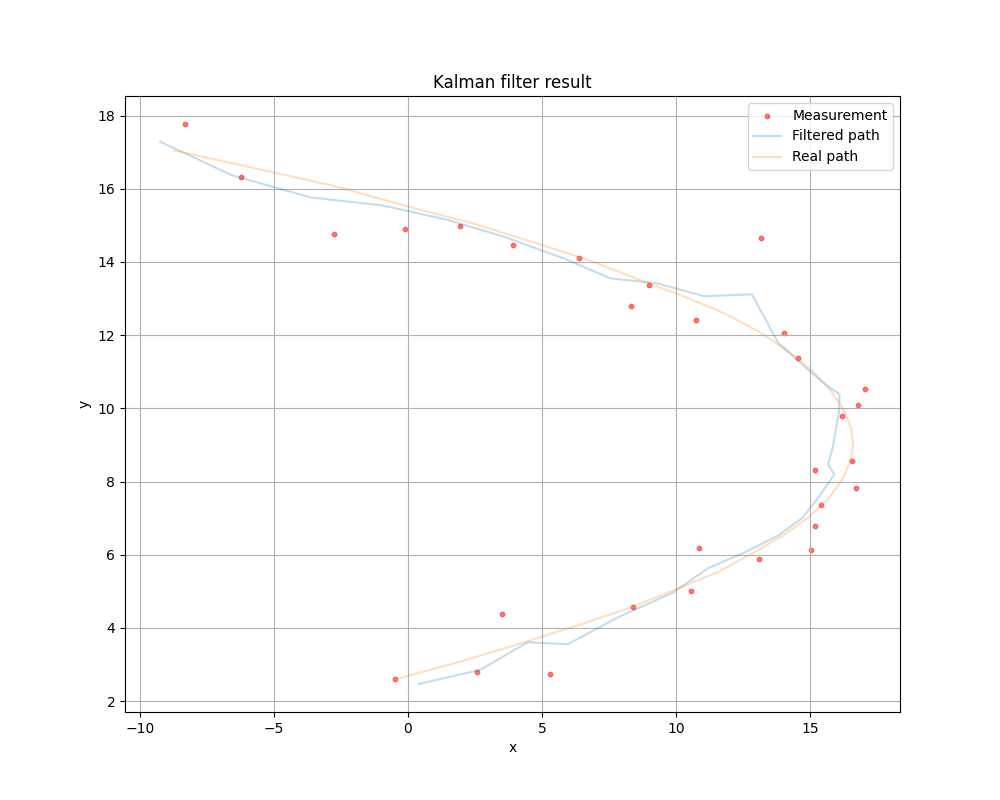
\includegraphics[width=0.4\textwidth]{./analyze1/Figure_4.png}
	}
\end{figure}
\begin{figure}[H]
	\centering
	\subfigure[$\rho=-0.99$]{
		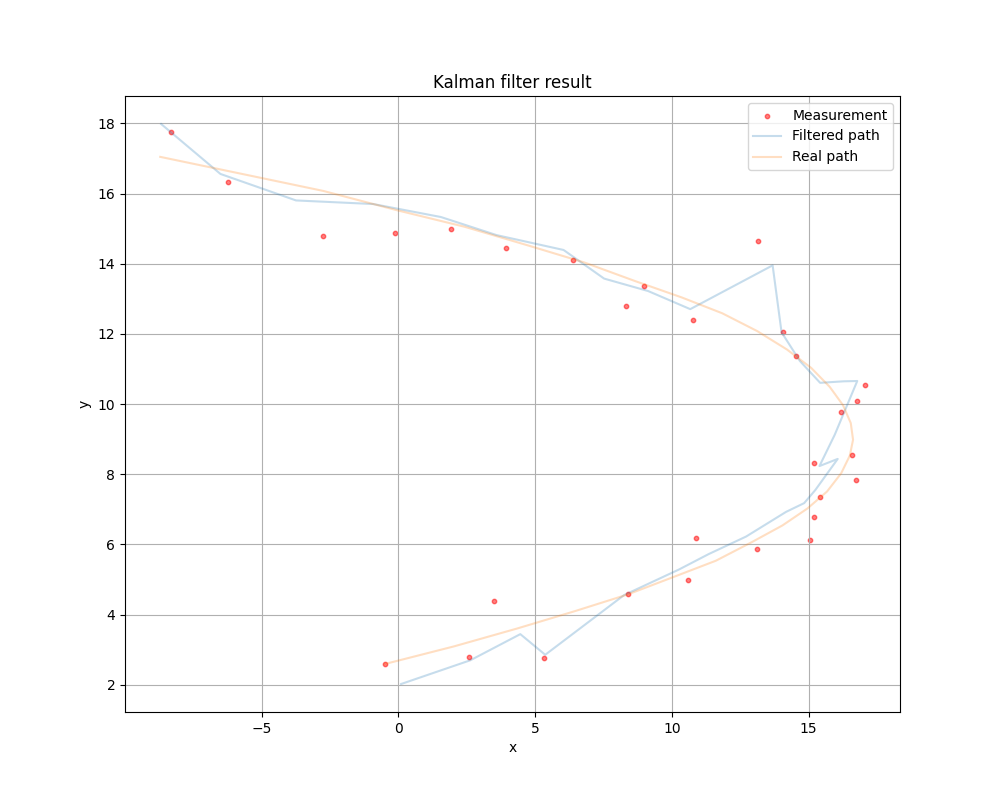
\includegraphics[width=0.4\textwidth]{./analyze1/Figure_5.png}
	}
\end{figure}

\subsubsection{Analyze 3}
分析 3 固定$R=\begin{bmatrix} 0.75 & 0 \\ 0 & 0.75 \end{bmatrix}$,調整$Q=\begin{bmatrix} 0.1 & 0 & \rho*0.1\\ 0 & 0.1 & \rho*0.1\\ \rho*0.1 & \rho*0.1 & 0.1 \end{bmatrix}$,設定條件$-1<\rho<1$之間依序調整驗證x y 和yaw 之間的相關性結果為非相關,因此結果無明顯誤差變化結果如圖所示。

\begin{figure}[H]
\centering
	\subfigure[$\rho=0.99$]{
	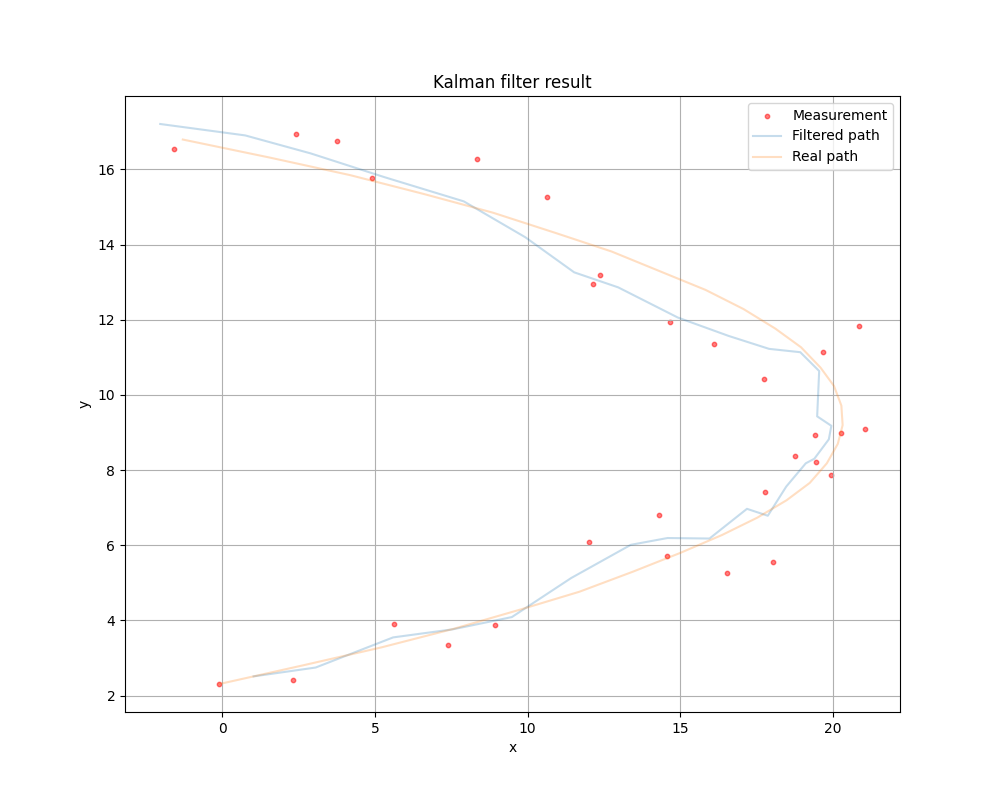
\includegraphics[width=0.4\textwidth]{./analyze2/Figure_1.png}
	}
	\subfigure[$\rho=0.5$]{
		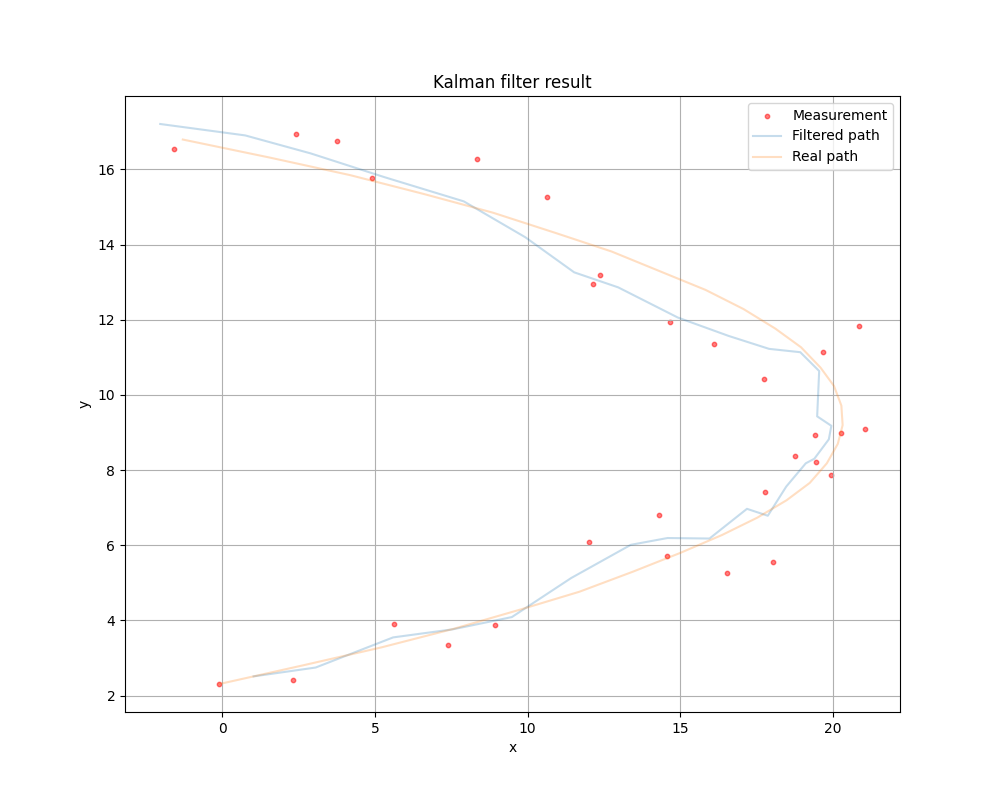
\includegraphics[width=0.4\textwidth]{./analyze2/Figure_2.png}
	}
\end{figure}

\begin{figure}[H]
\centering
	\subfigure[$\rho=0$]{
	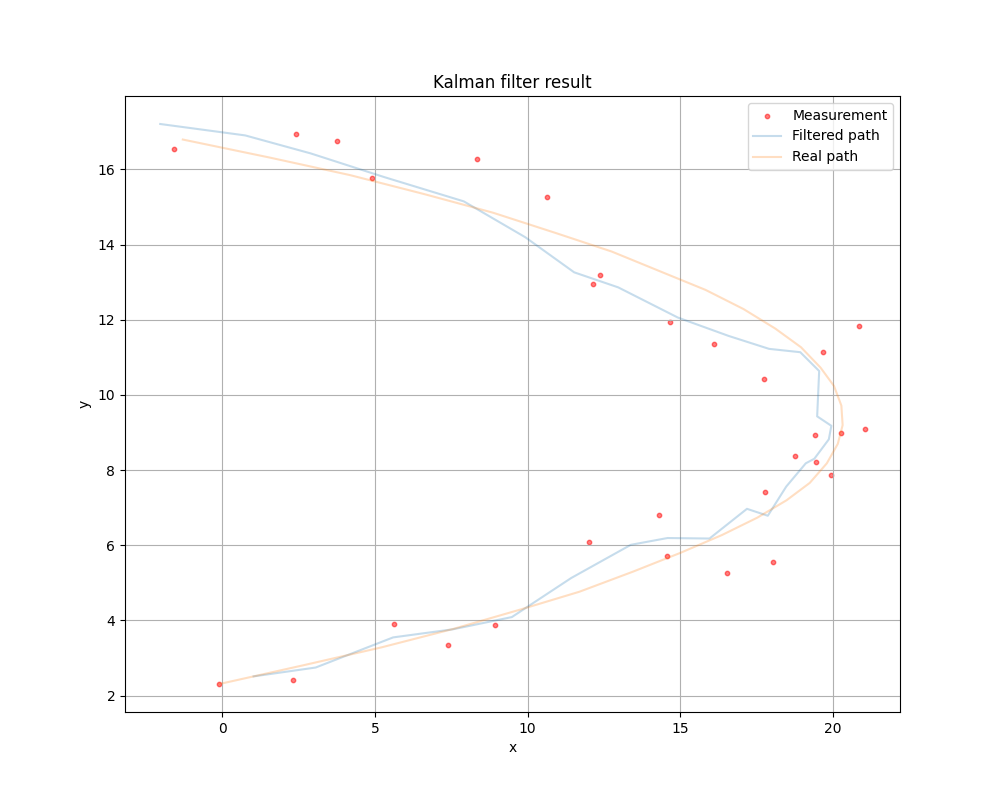
\includegraphics[width=0.4\textwidth]{./analyze2/Figure_3.png}
	}
	\subfigure[$\rho=-0.5$]{
		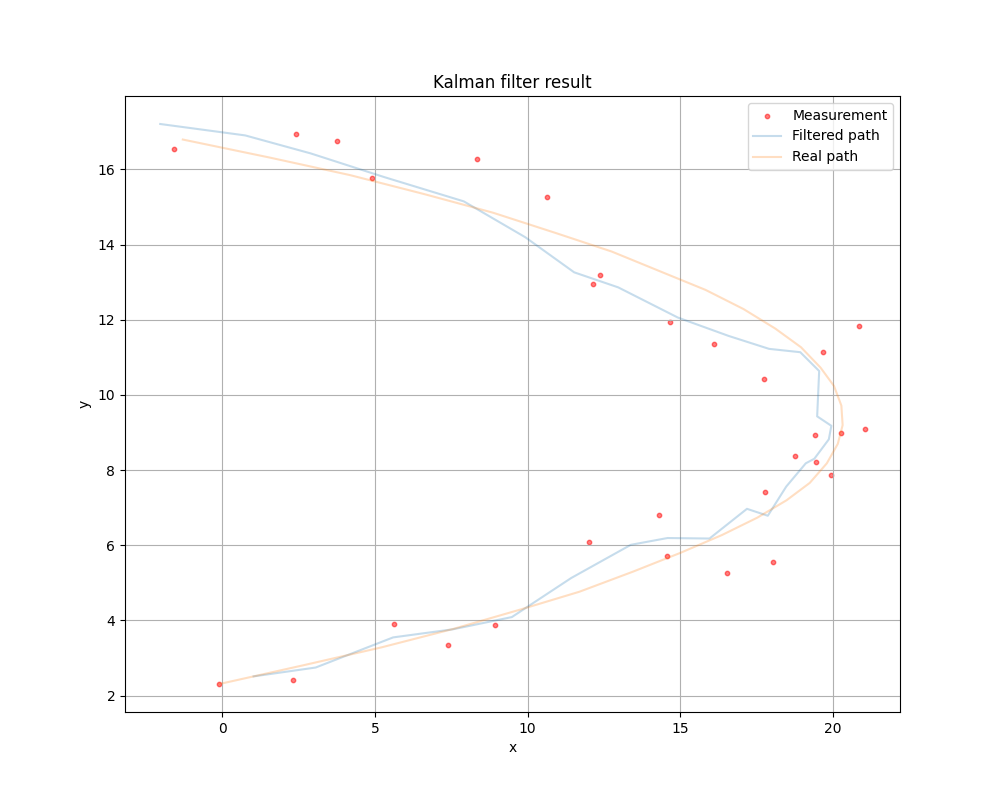
\includegraphics[width=0.4\textwidth]{./analyze2/Figure_4.png}
	}
\end{figure}

\begin{figure}[H]
\centering
	\subfigure[$\rho=0.99$]{
	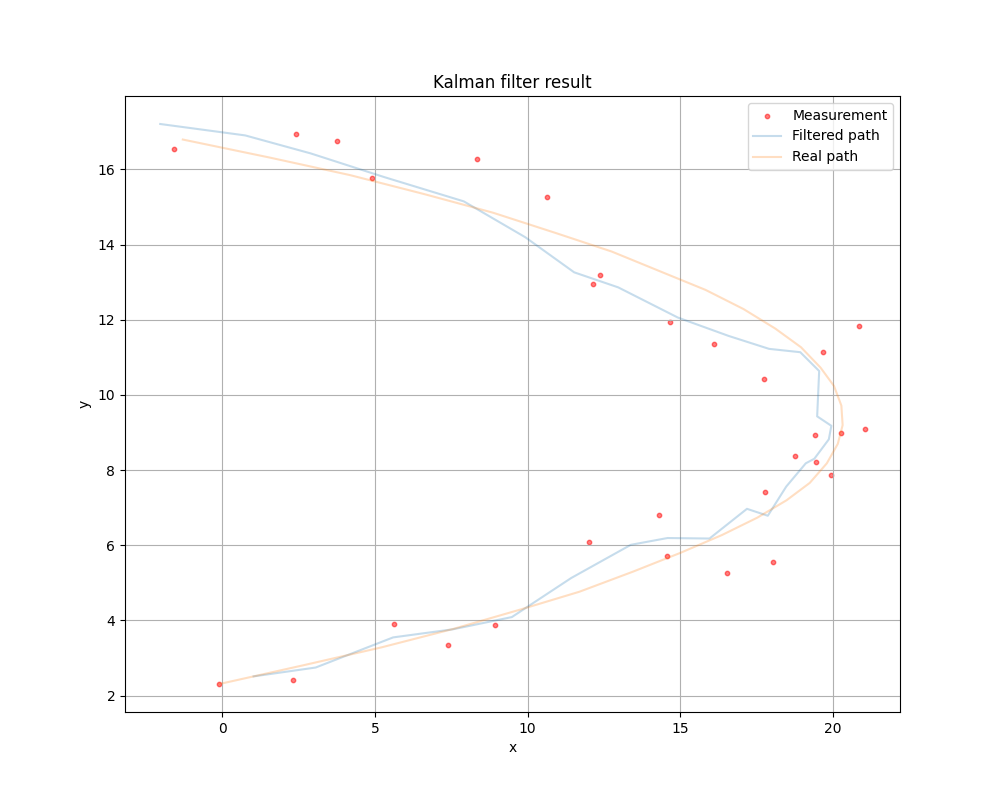
\includegraphics[width=0.4\textwidth]{./analyze2/Figure_5.png}
	}
\end{figure}

\subsection{Analyze 4}
	分析 4 固定$R=\begin{bmatrix} 0.75 & 0\\ 0 & 0.75 \end{bmatrix}$ , 調整$Q=\begin{bmatrix} 0.1 & \rho*0.1 0\\ \rho*0.1 & 0.1 & 0\\ 0 & 0 & 0.1 \end{bmatrix}$,設定條件$-1<\rho<1$之間依序驗證預測x y 之間的相關性,結果顯示$\rho=0.5$濾波效果較佳,結果如圖下所示。
\begin{figure}[H]
\centering
	\subfigure[$\rho=0.99$]{
	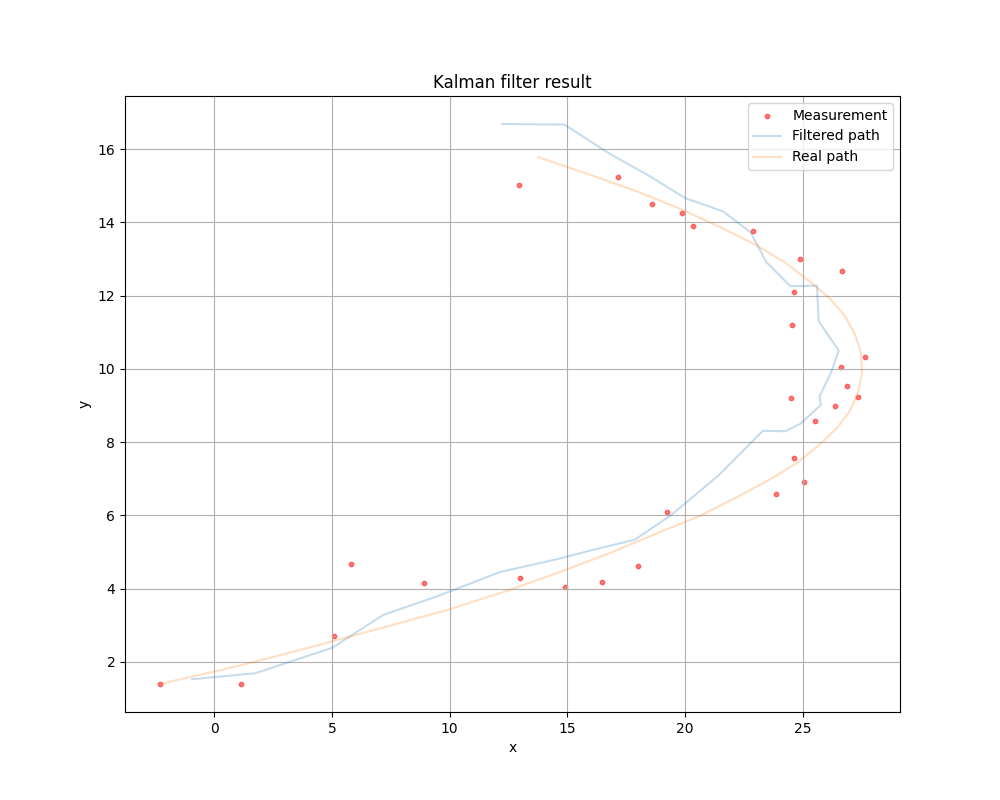
\includegraphics[width=0.4\textwidth]{./analyze3/Figure_1.png}
	}
	\subfigure[$\rho=0.5$]{
		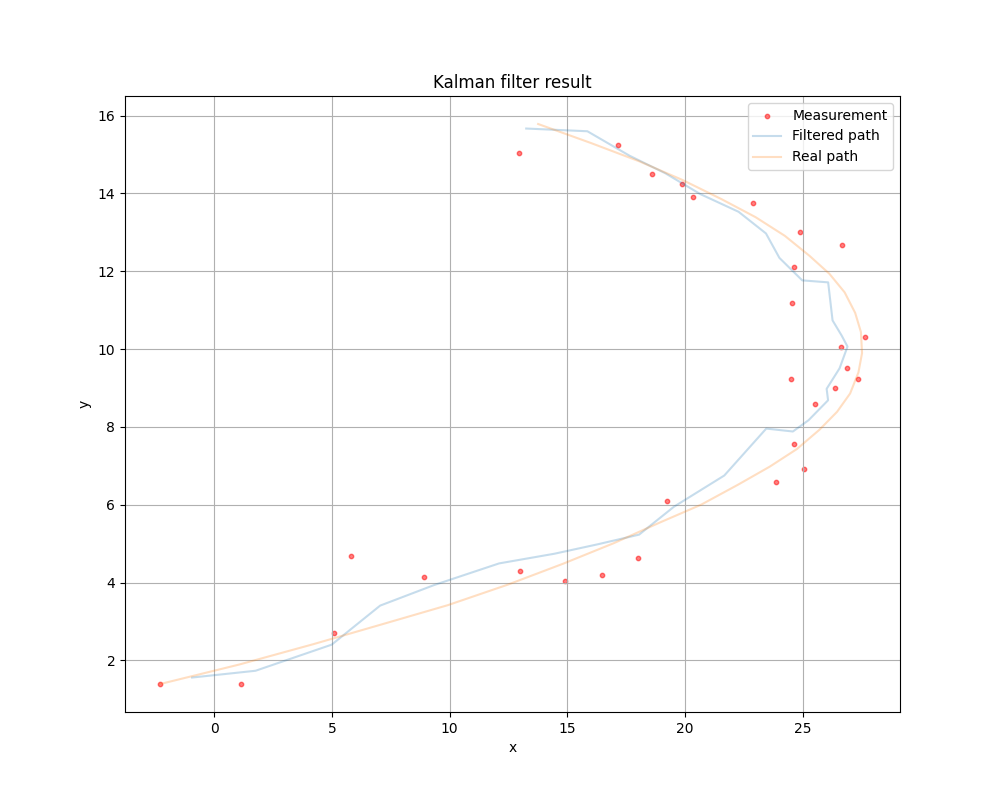
\includegraphics[width=0.4\textwidth]{./analyze3/Figure_2.png}
	}
\end{figure}

\begin{figure}[H]
\centering
	\subfigure[$\rho=0$]{
	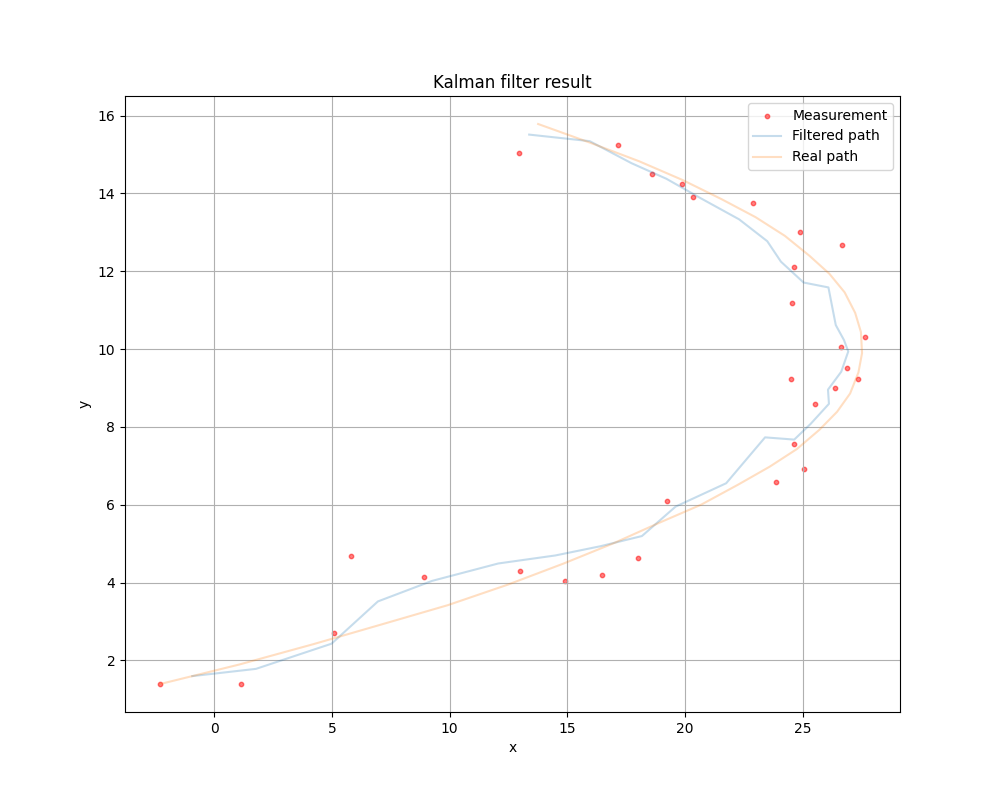
\includegraphics[width=0.4\textwidth]{./analyze3/Figure_3.png}
	}
	\subfigure[$\rho=-0.5$]{
		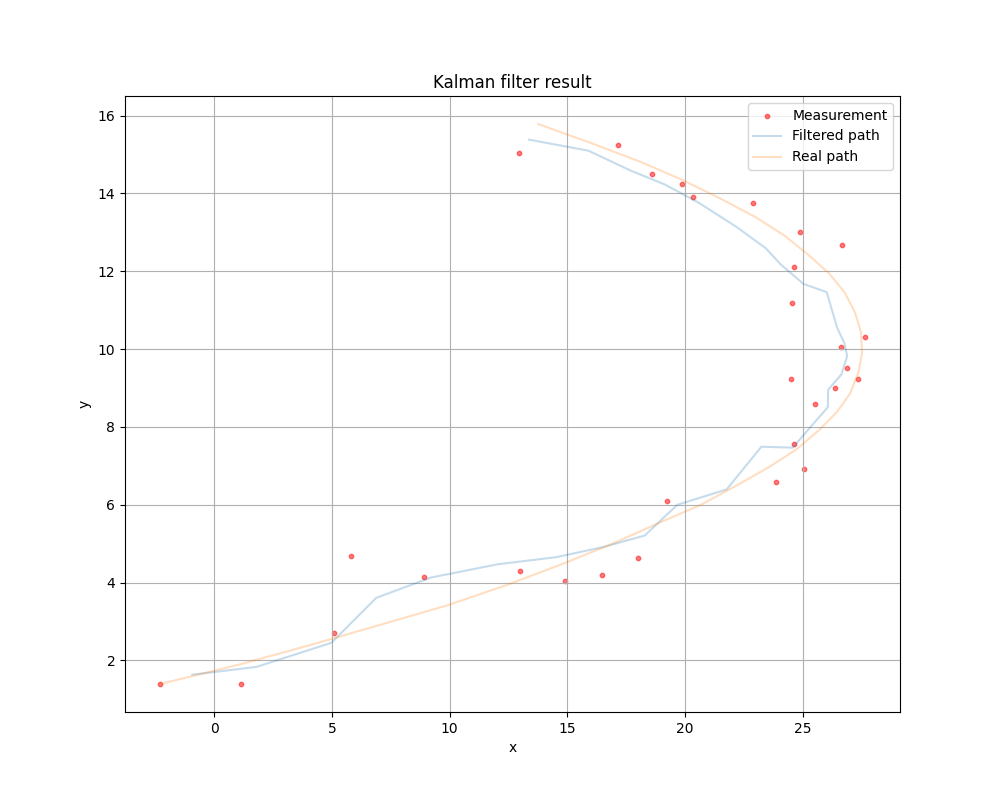
\includegraphics[width=0.4\textwidth]{./analyze3/Figure_4.png}
	}
\end{figure}

\begin{figure}[H]
\centering
	\subfigure[$\rho=0.99$]{
	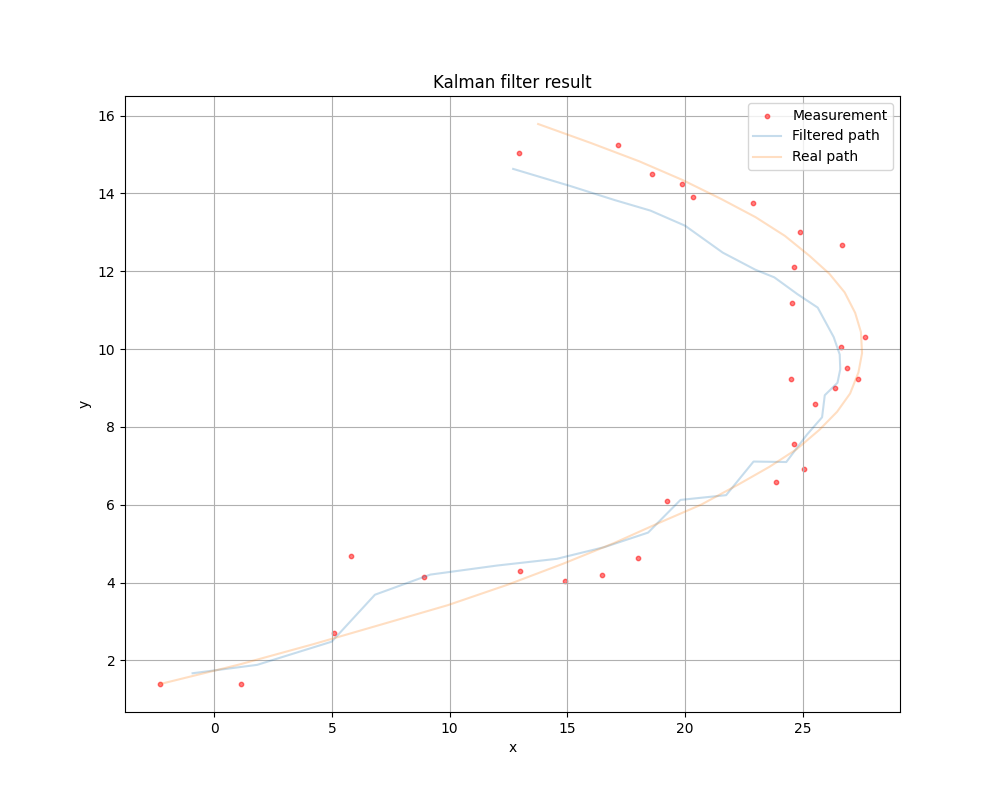
\includegraphics[width=0.4\textwidth]{./analyze3/Figure_5.png}
	}
\end{figure}

\subsubsection{Analyze Q R result} 
經分結果所設計的預測協方矩陣為$Q=\begin{bmatrix} 0.1 & 0.05 & 0\\0.05 & 0.1 & 0\\ 0 & 0 & 0.1 \end{bmatrix}$,則$R=\begin{bmatrix} 0.75 & 0\\ 0 & 0.75\end{bmatrix}$,經分析量測的unsertainty較大所以量測的weight較小,所以較依賴預測的狀態,結果如圖下示。

\begin{figure}[H]
\centering
	\subfigure[Q R設計結果]{
	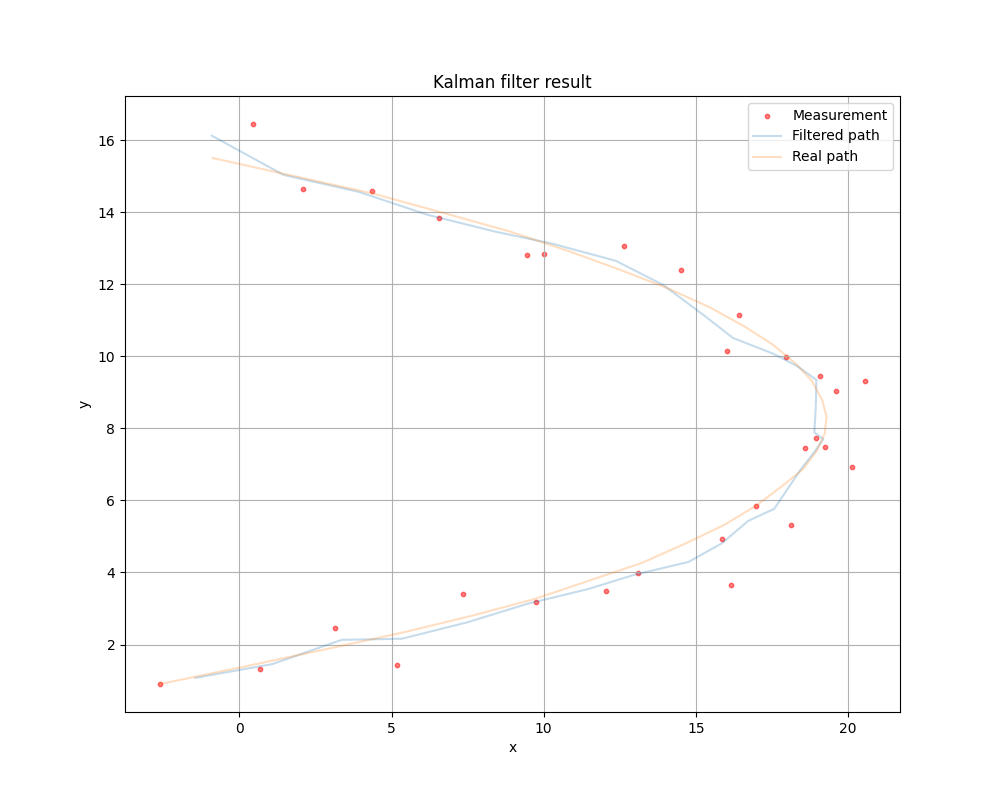
\includegraphics[width=0.4\textwidth]{./Figure_1.png}
	}
\end{figure}

\begin{thebibliography}{1}
 
\bibitem{1}
    Labbe, R. (2014). Kalman and bayesian filters in python. Chap, 7(246), 4.
\bibitem{2}
	Faragher, R. (2012). Understanding the basis of the kalman filter via a simple and intuitive derivation [lecture notes]. IEEE Signal processing magazine, 29(5), 128-132.

 
\end{thebibliography}


\end{document}
